\documentclass{article}
\usepackage[utf8]{inputenc}

\title{Echtzeitsysteme - Übung 1}
\author{Maximilian Nothnagel}
\date{}

\usepackage{natbib}
\usepackage{graphicx}
\usepackage{amsmath}

\begin{document}
	
	\maketitle
	
	\section*{1.1a) Model Fitting}
	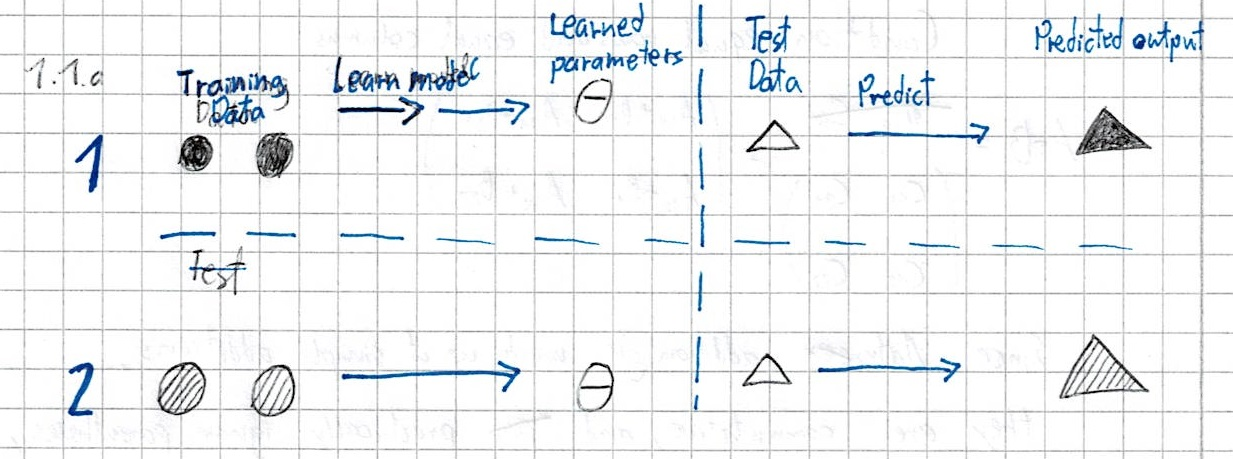
\includegraphics{1.1}\\
	Model 1 is being trained on filled circles, and as such assumes that the triangle is also to be filled, coming to an incorrect result.\\
	Model 2 is being trained on striped circles, and as such assumes that the triangle is also to be striped, coming to the correct conclusion.
	
	\section{1.2a) Matrix Algebra Refresher}
	\subsection{Multiplication}
	\begin{equation*} 
		A*B = 
		\begin{pmatrix}
			A_{1,1}*B_{1,1}+A_{2,1}*B_{1,2} & A_{1,1}*B_{2,1}+A_{2,1}*B_{2,2} \\
			A_{1,2}*B_{1,1}+A_{2,2}*B_{1,2} & A_{1,2}*B_{2,1}+A_{2,2}*B_{2,2}
		\end{pmatrix}
	\end{equation*}
	$A*B$ is defined only when Columns of B equal rows of A.\\
	\begin{equation*} 
		\begin{pmatrix}
			0 & 1 \\
			0 & 0
		\end{pmatrix}
		*
		\begin{pmatrix}
			0 & 0 \\
			1 & 0
		\end{pmatrix} 
		= 
		\begin{pmatrix}
			1 & 0 \\
			0 & 0
		\end{pmatrix}
	\end{equation*}
	BUT\\
	\begin{equation*} 
	\begin{pmatrix}
		0 & 0 \\
		1 & 0
	\end{pmatrix} 
	*
	\begin{pmatrix}
		0 & 1 \\
		0 & 0
	\end{pmatrix}
	= 
	\begin{pmatrix}
		0 & 0 \\
		0 & 1
	\end{pmatrix}
	\end{equation*}
	Matrixmultiplication is not Commutative.\\
	$A(B+C) = AB + AC$
	\begin{equation*} 
		\begin{pmatrix} %01
			0 & 1 \\	%00
			0 & 0
		\end{pmatrix} 
		*(
		\begin{pmatrix} %00
			0 & 0 \\	%10
			1 & 0
		\end{pmatrix}
		+ 
		\begin{pmatrix} %11
			1 & 1 \\	%11
			1 & 1
		\end{pmatrix}
		) =
		\begin{pmatrix} %10
			1 & 0 \\	%00
			0 & 0
		\end{pmatrix}
		+
		\begin{pmatrix} %11
			1 & 1 \\	%00
			0 & 0
		\end{pmatrix}
		=
		\begin{pmatrix} %21
			2 & 1 \\	%00
			0 & 0
		\end{pmatrix} 
		\end{equation*}
		\begin{equation*}
	  	\begin{pmatrix} %01
	  		0 & 1 \\	%00
	  		0 & 0
	  	\end{pmatrix} 
  		*
  		\begin{pmatrix} %11
  			1 & 1 \\	%21
  			2 & 1
  		\end{pmatrix} 
  		=
  		\begin{pmatrix} %21
  			2 & 1 \\	%00
  			0 & 0
  		\end{pmatrix} 
	\end{equation*}
	Matrixmultiplication is Distributive.\\
		
		
	$(A*B)*C = A*(B*C)$
	\begin{equation*} 
		(
		\begin{pmatrix} %01
			0 & 1 \\	%00
			0 & 0
		\end{pmatrix} 
		*
		\begin{pmatrix} %00
			0 & 0 \\	%10
			1 & 0
		\end{pmatrix}
		) *
		\begin{pmatrix} %11
			1 & 1 \\	%11
			1 & 1
		\end{pmatrix}
		=
		\begin{pmatrix} %11
			1 & 1 \\	%00
			0 & 0
		\end{pmatrix}	
	\end{equation*}
	\begin{equation*} 	
		\begin{pmatrix} %01
			0 & 1 \\	%00
			0 & 0
		\end{pmatrix} 
		* (
		\begin{pmatrix} %00
			0 & 0 \\	%10
			1 & 0
		\end{pmatrix}
		 *
		\begin{pmatrix} %11
			1 & 1 \\	%11
			1 & 1
		\end{pmatrix}
		) =
		\begin{pmatrix} %11
			1 & 1 \\	%00
			0 & 0
		\end{pmatrix}	
	\end{equation*}
	\subsection{Addition}
	Since matrix-addition is made up of simple additions, they are commutative and practically ignore parentheses, so are also distributive and associative.\\
	The condition for any matrix-addition is that the matrices have both equal rows and columns.\\
	\begin{equation*} 
		A_{2,2}+B_{2,2}=
		\begin{pmatrix}
			C_{1,1} & C_{2,1} \\
			C_{1,2} & C_{2,2}
		\end{pmatrix}
		=
	\begin{pmatrix}
		A_{1,1}+B_{1,1} & A_{2,1}+B_{2,1} \\
		A_{1,2}+B_{1,2} & A_{2,2}+B_{2,2}
	\end{pmatrix}
	\end{equation*}

\section{1.2b) Matrix Inversion}
	$A^{-1} =$ \begin{equation*}
		\begin{pmatrix}
			 1 & 0 & 0 \\
			-1 & 1 & 0 \\
			 0 & 0 & 1
		\end{pmatrix}
	\end{equation*} \\
	...Via Gauß-Jordan. Under the condition that $a=b=d=0; c=1$\\
	\begin{equation*}
		\begin{pmatrix}
			2 & 2 &  3 \\
			0 & 1 &  0 \\
			8 & 3 & 12
		\end{pmatrix}
	\end{equation*}
	Is not invertable, since it's Determinant $Det = 0$.
	
	\section{1.2c) Matrix Pseudoinverse}
	Left: $A^\# * A = (A^T * A)^{-1} * A^T$ \\
	Right: $A * A^\# = A * A^T (A * A^T)^{-1}$\\
	Since $A_{2x3}$ has more rows than columns, the left Moore-Penrose exists.\\
	The equation is: $A^\#_{3x2} * A = (A^T_{3x2} * A_{2x3})^{-1}_{2x2} * A^T_{3x2}$
	
	\section{1.2d) Basis Transformation}
	Vector with new Basis $v^* = T^{-1} * v$\\\\
	1) $T_v = E^{-1} = \begin{pmatrix}
		1 & 0\\
		0 & 1
	\end{pmatrix};
	T_w = B^{-1} = \begin{pmatrix}
		 2 & -1.5\\
		-1 & 1
	\end{pmatrix}$\\\\
	2) $2 * \begin{bmatrix}
		2 \\
		-1
	\end{bmatrix}
	+ 5 * \begin{bmatrix}
		-1,5 \\
		 1
	\end{bmatrix}
	 = \begin{bmatrix}
	 	-3,5 \\
	 	 3
	 \end{bmatrix} = v^*$
\end{document}
